
%% 多种区域故障类型考虑
%% 多种问题讨论 丰富内容
%% 虚拟化网络中的故障 故障概率考虑
%% NFV 和电网结合的头图修改和图的标题 概念。把具体问题放进去,用visio画一个好看的。 使用NFV的专用术语。看NFV的论文 抄一个intro。
%% 第三作者修改 
%% 疯狂的套nfv
%% Fig 1 arch and base 的电力通信网

%% MANO接受业务请求,里面是业务链条 根据照片修改
%% 根据上一个论文意见看看有没有论文的问题


%% bare_jrnl.tex
%% V1.4b
%% 2015/08/26
%% by Michael Shell
%% see http://www.michaelshell.org/
%% for current contact information.
%%
%% This is a skeleton file demonstrating the use of IEEEtran.cls
%% (requires IEEEtran.cls version 1.8b or later) with an IEEE
%% journal paper.
%%
%% Support sites:
%% http://www.michaelshell.org/tex/ieeetran/
%% http://www.ctan.org/pkg/ieeetran
%% and
%% http://www.ieee.org/

%%*************************************************************************
%% Legal Notice:
%% This code is offered as-is without any warranty either expressed or
%% implied; without even the implied warranty of MERCHANTABILITY or
%% FITNESS FOR A PARTICULAR PURPOSE! 
%% User assumes all risk.
%% In no event shall the IEEE or any contributor to this code be liable for
%% any damages or losses, including, but not limited to, incidental,
%% consequential, or any other damages, resulting from the use or misuse
%% of any information contained here.
%%
%% All comments are the opinions of their respective authors and are not
%% necessarily endorsed by the IEEE.
%%
%% This work is distributed under the LaTeX Project Public License (LPPL)
%% ( http://www.latex-project.org/ ) version 1.3, and may be freely used,
%% distributed and modified. A copy of the LPPL, version 1.3, is included
%% in the base LaTeX documentation of all distributions of LaTeX released
%% 2003/12/01 or later.
%% Retain all contribution notices and credits.
%% ** Modified files should be clearly indicated as such, including  **
%% ** renaming them and changing author support contact information. **
%%*************************************************************************


% *** Authors should verify (and, if needed, correct) their LaTeX system  ***
% *** with the testflow diagnostic prior to trusting their LaTeX platform ***
% *** with production work. The IEEE's font choices and paper sizes can   ***
% *** trigger bugs that do not appear when using other class files.       ***                          ***
% The testflow support page is at:
% http://www.michaelshell.org/tex/testflow/



\documentclass[journal]{IEEEtran}
\usepackage{graphicx}
\usepackage[justification=centering]{caption}
\usepackage{CJK}
\usepackage[top=2cm, bottom=2cm, left=2cm, right=2cm]{geometry}
\usepackage{algorithm}
\usepackage{algorithmicx}
\usepackage{algpseudocode}
\usepackage{amsmath}
\usepackage{xcolor}%???????  
\usepackage{colortbl,booktabs}%?????????*rule  
 \usepackage{booktabs}
 \usepackage{subfigure}
 \usepackage{verbatim}
 \usepackage{pgfplots}
\usepackage{tikz}    
\usetikzlibrary{arrows,shapes,chains}  

\floatname{algorithm}{Algorithm}
\renewcommand{\algorithmicrequire}{\textbf{Input:}}
\renewcommand{\algorithmicensure}{\textbf{Output:}}
%
% If IEEEtran.cls has not been installed into the LaTeX system files,
% manually specify the path to it like:
% \documentclass[journal]{../sty/IEEEtran}





% Some very useful LaTeX packages include:
% (uncomment the ones you want to load)


% *** MISC UTILITY PACKAGES ***
%
%\usepackage{ifpdf}
% Heiko Oberdiek's ifpdf.sty is very useful if you need conditional
% compilation based on whether the output is pdf or dvi.
% usage:
% \ifpdf
%   % pdf code
% \else
%   % dvi code
% \fi
% The latest version of ifpdf.sty can be obtained from:
% http://www.ctan.org/pkg/ifpdf
% Also, note that IEEEtran.cls V1.7 and later provides a builtin
% \ifCLASSINFOpdf conditional that works the same way.
% When switching from latex to pdflatex and vice-versa, the compiler may
% have to be run twice to clear warning/error messages.






% *** CITATION PACKAGES ***
%
%\usepackage{cite}
% cite.sty was written by Donald Arseneau
% V1.6 and later of IEEEtran pre-defines the format of the cite.sty package
% \cite{} output to follow that of the IEEE. Loading the cite package will
% result in citation numbers being automatically sorted and properly
% "compressed/ranged". e.g., [1], [9], [2], [7], [5], [6] without using
% cite.sty will become [1], [2], [5]--[7], [9] using cite.sty. cite.sty's
% \cite will automatically add leading space, if needed. Use cite.sty's
% noadjust option (cite.sty V3.8 and later) if you want to turn this off
% such as if a citation ever needs to be enclosed in parenthesis.
% cite.sty is already installed on most LaTeX systems. Be sure and use
% version 5.0 (2009-03-20) and later if using hyperref.sty.
% The latest version can be obtained at:
% http://www.ctan.org/pkg/cite
% The documentation is contained in the cite.sty file itself.






% *** GRAPHICS RELATED PACKAGES ***
%
\ifCLASSINFOpdf
  % \usepackage[pdftex]{graphicx}
  % declare the path(s) where your graphic files are
  % \graphicspath{{../pdf/}{../jpeg/}}
  % and their extensions so you won't have to specify these with
  % every instance of \includegraphics
  % \DeclareGraphicsExtensions{.pdf,.jpeg,.png}
\else
  % or other class option (dvipsone, dvipdf, if not using dvips). graphicx
  % will default to the driver specified in the system graphics.cfg if no
  % driver is specified.
  % \usepackage[dvips]{graphicx}
  % declare the path(s) where your graphic files are
  % \graphicspath{{../eps/}}
  % and their extensions so you won't have to specify these with
  % every instance of \includegraphics
  % \DeclareGraphicsExtensions{.eps}
\fi
% graphicx was written by David Carlisle and Sebastian Rahtz. It is
% required if you want graphics, photos, etc. graphicx.sty is already
% installed on most LaTeX systems. The latest version and documentation
% can be obtained at: 
% http://www.ctan.org/pkg/graphicx
% Another good source of documentation is "Using Imported Graphics in
% LaTeX2e" by Keith Reckdahl which can be found at:
% http://www.ctan.org/pkg/epslatex
%
% latex, and pdflatex in dvi mode, support graphics in encapsulated
% postscript (.eps) format. pdflatex in pdf mode supports graphics
% in .pdf, .jpeg, .png and .mps (metapost) formats. Users should ensure
% that all non-photo figures use a vector format (.eps, .pdf, .mps) and
% not a bitmapped formats (.jpeg, .png). The IEEE frowns on bitmapped formats
% which can result in "jaggedy"/blurry rendering of lines and letters as
% well as large increases in file sizes.
%
% You can find documentation about the pdfTeX application at:
% http://www.tug.org/applications/pdftex





% *** MATH PACKAGES ***
%
%\usepackage{amsmath}
% A popular package from the American Mathematical Society that provides
% many useful and powerful commands for dealing with mathematics.
%
% Note that the amsmath package sets \interdisplaylinepenalty to 10000
% thus preventing page breaks from occurring within multiline equations. Use:
%\interdisplaylinepenalty=2500
% after loading amsmath to restore such page breaks as IEEEtran.cls normally
% does. amsmath.sty is already installed on most LaTeX systems. The latest
% version and documentation can be obtained at:
% http://www.ctan.org/pkg/amsmath





% *** SPECIALIZED LIST PACKAGES ***
%
%\usepackage{algorithmic}
% algorithmic.sty was written by Peter Williams and Rogerio Brito.
% This package provides an algorithmic environment fo describing algorithms.
% You can use the algorithmic environment in-text or within a figure
% environment to provide for a floating algorithm. Do NOT use the algorithm
% floating environment provided by algorithm.sty (by the same authors) or
% algorithm2e.sty (by Christophe Fiorio) as the IEEE does not use dedicated
% algorithm float types and packages that provide these will not provide
% correct IEEE style captions. The latest version and documentation of
% algorithmic.sty can be obtained at:
% http://www.ctan.org/pkg/algorithms
% Also of interest may be the (relatively newer and more customizable)
% algorithmicx.sty package by Szasz Janos:
% http://www.ctan.org/pkg/algorithmicx




% *** ALIGNMENT PACKAGES ***
%
%\usepackage{array}
% Frank Mittelbach's and David Carlisle's array.sty patches and improves
% the standard LaTeX2e array and tabular environments to provide better
% appearance and additional user controls. As the default LaTeX2e table
% generation code is lacking to the point of almost being broken with
% respect to the quality of the end results, all users are strongly
% advised to use an enhanced (at the very least that provided by array.sty)
% set of table tools. array.sty is already installed on most systems. The
% latest version and documentation can be obtained at:
% http://www.ctan.org/pkg/array


% IEEEtran contains the IEEEeqnarray family of commands that can be used to
% generate multiline equations as well as matrices, tables, etc., of high
% quality.




% *** SUBFIGURE PACKAGES ***
%\ifCLASSOPTIONcompsoc
%  \usepackage[caption=false,font=normalsize,labelfont=sf,textfont=sf]{subfig}
%\else
%  \usepackage[caption=false,font=footnotesize]{subfig}
%\fi
% subfig.sty, written by Steven Douglas Cochran, is the modern replacement
% for subfigure.sty, the latter of which is no longer maintained and is
% incompatible with some LaTeX packages including fixltx2e. However,
% subfig.sty requires and automatically loads Axel Sommerfeldt's caption.sty
% which will override IEEEtran.cls' handling of captions and this will result
% in non-IEEE style figure/table captions. To prevent this problem, be sure
% and invoke subfig.sty's "caption=false" package option (available since
% subfig.sty version 1.3, 2005/06/28) as this is will preserve IEEEtran.cls
% handling of captions.
% Note that the Computer Society format requires a larger sans serif font
% than the serif footnote size font used in traditional IEEE formatting
% and thus the need to invoke different subfig.sty package options depending
% on whether compsoc mode has been enabled.
%
% The latest version and documentation of subfig.sty can be obtained at:
% http://www.ctan.org/pkg/subfig




% *** FLOAT PACKAGES ***
%
%\usepackage{fixltx2e}
% fixltx2e, the successor to the earlier fix2col.sty, was written by
% Frank Mittelbach and David Carlisle. This package corrects a few problems
% in the LaTeX2e kernel, the most notable of which is that in current
% LaTeX2e releases, the ordering of single and double column floats is not
% guaranteed to be preserved. Thus, an unpatched LaTeX2e can allow a
% single column figure to be placed prior to an earlier double column
% figure.
% Be aware that LaTeX2e kernels dated 2015 and later have fixltx2e.sty's
% corrections already built into the system in which case a warning will
% be issued if an attempt is made to load fixltx2e.sty as it is no longer
% needed.
% The latest version and documentation can be found at:
% http://www.ctan.org/pkg/fixltx2e


%\usepackage{stfloats}
% stfloats.sty was written by Sigitas Tolusis. This package gives LaTeX2e
% the ability to do double column floats at the bottom of the page as well
% as the top. (e.g., "\begin{figure*}[!b]" is not normally possible in
% LaTeX2e). It also provides a command:
%\fnbelowfloat
% to enable the placement of footnotes below bottom floats (the standard
% LaTeX2e kernel puts them above bottom floats). This is an invasive package
% which rewrites many portions of the LaTeX2e float routines. It may not work
% with other packages that modify the LaTeX2e float routines. The latest
% version and documentation can be obtained at:
% http://www.ctan.org/pkg/stfloats
% Do not use the stfloats baselinefloat ability as the IEEE does not allow
% \baselineskip to stretch. Authors submitting work to the IEEE should note
% that the IEEE rarely uses double column equations and that authors should try
% to avoid such use. Do not be tempted to use the cuted.sty or midfloat.sty
% packages (also by Sigitas Tolusis) as the IEEE does not format its papers in
% such ways.
% Do not attempt to use stfloats with fixltx2e as they are incompatible.
% Instead, use Morten Hogholm'a dblfloatfix which combines the features
% of both fixltx2e and stfloats:
%
% \usepackage{dblfloatfix}
% The latest version can be found at:
% http://www.ctan.org/pkg/dblfloatfix




%\ifCLASSOPTIONcaptionsoff
%  \usepackage[nomarkers]{endfloat}
% \let\MYoriglatexcaption\caption
% \renewcommand{\caption}[2][\relax]{\MYoriglatexcaption[#2]{#2}}
%\fi
% endfloat.sty was written by James Darrell McCauley, Jeff Goldberg and 
% Axel Sommerfeldt. This package may be useful when used in conjunction with 
% IEEEtran.cls'  captionsoff option. Some IEEE journals/societies require that
% submissions have lists of figures/tables at the end of the paper and that
% figures/tables without any captions are placed on a page by themselves at
% the end of the document. If needed, the draftcls IEEEtran class option or
% \CLASSINPUTbaselinestretch interface can be used to increase the line
% spacing as well. Be sure and use the nomarkers option of endfloat to
% prevent endfloat from "marking" where the figures would have been placed
% in the text. The two hack lines of code above are a slight modification of
% that suggested by in the endfloat docs (section 8.4.1) to ensure that
% the full captions always appear in the list of figures/tables - even if
% the user used the short optional argument of \caption[]{}.
% IEEE papers do not typically make use of \caption[]'s optional argument,
% so this should not be an issue. A similar trick can be used to disable
% captions of packages such as subFsty that lack options to turn off
% the subcaptions:
% For subfig.sty:
% \let\MYorigsubfloat\subfloat
% \renewcommand{\subfloat}[2][\relax]{\MYorigsubfloat[]{#2}}
% However, the above trick will not work if both optional arguments of
% the \subfloat command are used. Furthermore, there needs to be a
% description of each subfigure *somewhere* and endfloat does not add
% subfigure captions to its list of figures. Thus, the best approach is to
% avoid the use of subfigure captions (many IEEE journals avoid them anyway)
% and instead reference/explain all the subfigures within the main caption.
% The latest version of endfloat.sty and its documentation can obtained at:
% http://www.ctan.org/pkg/endfloat
%
% The IEEEtran \ifCLASSOPTIONcaptionsoff conditional can also be used
% later in the document, say, to conditionally put the References on a 
% page by themselves.




% *** PDF, URL AND HYPERLINK PACKAGES ***
%
%\usepackage{url}
% url.sty was written by Donald Arseneau. It provides better support for
% handling and breaking URLs. url.sty is already installed on most LaTeX
% systems. The latest version and documentation can be obtained at:
% http://www.ctan.org/pkg/url
% Basically, \url{my_url_here}.




% *** Do not adjust lengths that control margins, column widths, etc. ***
% *** Do not use packages that alter fonts (such as pslatex).         ***
% There should be no need to do such things with IEEEtran.cls V1.6 and later.
% (Unless specifically asked to do so by the journal or conference you plan
% to submit to, of course. )


% correct bad hyphenation here
\hyphenation{op-tical net-works semi-conduc-tor}


\begin{document}
%
% paper title
% Titles are generally capitalized except for words such as a, an, and, as,
% at, but, by, for, in, nor, of, on, or, the, to and up, which are usually
% not capitalized unless they are the first or last word of the title.
% Linebreaks \\ can be used within to get better formatting as desired.
% Do not put math or special symbols in the title.
\title{A Sampling Point Based Fault Tolerant Algorithm for NFV based Smart Grid Communication Network}
%
%
% author names and IEEE memberships
% note positions of commas and nonbreaking spaces ( ~ ) LaTeX will not break
% a structure at a ~ so this keeps an author's name from being broken across
% two lines.
% use \thanks{} to gain access to the first footnote area
% a separate \thanks must be used for each paragraph as LaTeX2e's \thanks
% was not built to handle multiple paragraphs
%

\author{
Lanlan~Rui, Xia~Zhen, Jiawen~Li, Xuesong~Qiu\\
State Key Laboratory of Networking and Switching Technology\\
Beijing University of Posts and Telecommunications\\
Beijing 100876, China\\
E-mail: \{llrui, xalyf, jiawen, xsqiu\}@bupt.edu.cn\\
}

% note the % following the last \IEEEmembership and also \thanks - 
% these prevent an unwanted space from occurring between the last author name
% and the end of the author line. i.e., if you had this:
% 
% \author{....lastname \thanks{...} \thanks{...} }
%                     ^------------^------------^----Do not want these spaces!
%
% a space would be appended to the last name and could cause every name on that
% line to be shifted left slightly. This is one of those "LaTeX things". For
% instance, "\textbf{A} \textbf{B}" will typeset as "A B" not "AB". To get
% "AB" then you have to do: "\textbf{A}\textbf{B}"
% \thanks is no different in this regard, so shield the last } of each \thanks
% that ends a line with a % and do not let a space in before the next \thanks.
% Spaces after \IEEEmembership other than the last one are OK (and needed) as
% you are supposed to have spaces between the names. For what it is worth,
% this is a minor point as most people would not even notice if the said evil
% space somehow managed to creep in.




% The only time the second header will appear is for the odd numbered pages
% after the title page when using the twoside option.
% 
% *** Note that you probably will NOT want to include the author's ***
% *** name in the headers of peer review papers.                   ***
% You can use \ifCLASSOPTIONpeerreview for conditional compilation here if
% you desire.




% If you want to put a publisher's ID mark on the page you can do it like
% this:
%\IEEEpubid{0000--0000/00\$00.00~\copyright~2015 IEEE}
% Remember, if you use this you must call \IEEEpubidadjcol in the second
% column for its text to clear the IEEEpubid mark.



% use for special paper notices
%\IEEEspecialpapernotice{(Invited Paper)}




% make the title area
\maketitle

% As a general rule, do not put math, special symbols or citations
% in the abstract or keywords.
\begin{abstract}

In this paper, we study the smart grid communication network based on the regional failure and network design irrationality in the network function virtualization (NFV). We propose a network backup algorithm: SPA (Sampling Point Based Fault Tolerant Algorithm). The goal of SPA is to promote the robustness of the entire network to regional failures.
\par In simulation experiments, this paper analyzes network modeling and topology features of the NFV three-tier smart grid communication network. We use LSRA (Landmark-based Source Routing Algorithm) and PRFAA (Probabilistic Region Failure-Aware Algorithm) as control groups which the smart grid communication network widely uses. SPA simulates random area faults through node sampling and can perform more accurate node backups. The simulation results which we performed in this article show that SPA is better than the rest of the algorithms. 
\end{abstract}
% Note that keywords are not normally used for peerreview papers.
\begin{IEEEkeywords}
smart grid communication network, NFV, Regional Fault, Backup Algorithm
\end{IEEEkeywords}





% For peer review papers, you can put extra information on the cover
% page as needed:
% \ifCLASSOPTIONpeerreview
% \begin{center} \bfseries EDICS Category: 3-BBND \end{center}
% \fi
%
% For peerreview papers, this IEEEtran command inserts a page break and
% creates the second title. It will be ignored for other modes.
\IEEEpeerreviewmaketitle
\pgfplotsset{every axis legend/.style={%
cells={anchor=west},
inner xsep=3pt,inner ysep=2pt,nodes={inner sep=2pt,text depth=0.15em},
anchor=north east,%
shape=rectangle,%
%fill=white,%
draw=black,
at={(0.98,0.98)}
}}



\section{Introduction}
% The very first letter is a 2 line initial drop letter followed
% by the rest of the first word in caps.
% 
% form to use if the first word consists of a single letter:
% \IEEEPARstart{A}{demo} file is ....
% 
% form to use if you need the single drop letter followed by
% normal text (unknown if ever used by the IEEE):
% \IEEEPARstart{A}{}demo file is ....
% 
% Some journals put the first two words in caps:
% \IEEEPARstart{T}{his demo} file is ....
% 
% Here we have the typical use of a "T" for an initial drop letter
% and "HIS" in caps to complete the first word.
% and "HIS" in caps to complete the first word.

\IEEEPARstart{W}{ith} the development of smart grid communication network technology, the requirements of users for power reliability have been continuously improved. Smart grid has become an inevitable trend in the development of smart grid communication network technology and an inevitable choice for social and economic development [1]. Smart grids are the source and driving force for grid development. It is also a key area of technology for smart grid construction. Therefore, further study about the reliability of smart grids are still essential.
\begin{figure}
\centering
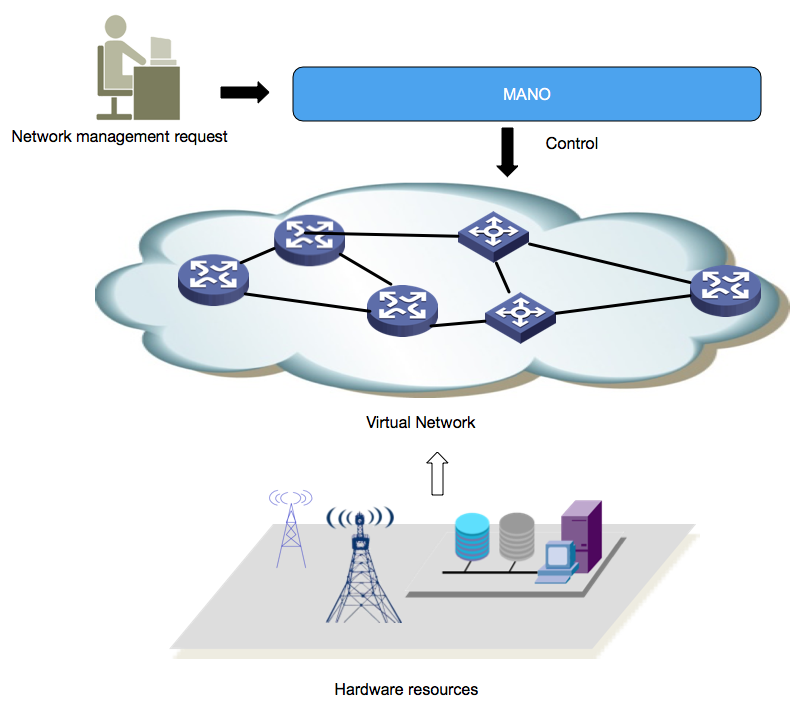
\includegraphics [width=3.4in]{NV-1}\ \caption{the architecture of NFV based Smart Grid CommunicationNetwork}
\end{figure}
\par Although it is difficult to predict the random occurrence and scale of such disasters, the consequences can still be mitigated by deploying additional resources in failures in large-scale disaster areas [2]. A typical way for network operators to provide service continuity in the event of a large-scale disaster is to allocate additional backup optical links because this will create more alternative paths. However, since both the main optical link and the backup optical link are susceptible to the same impact caused by the disaster, adding network redundancy on the optical physical medium is considered to be spatially inefficient and very expensive [3].
\par This paper explores the problem of regional faults in the NFV. NFV deals with the virtualization of network functions typically performed by dedicated hardware devices. Industry and academia are using NFV to promote innovation and provide flexibility in network management [4].

\par In NFV, the network is divided into the hardware resources (HS) and virtual network (VN) shown in Fig.1 [5]. HS contains specific network components provided by infrastructure provider, such as the power communication network and the smart grid communication network [6]. MANO (NFV Management and Orchestration) is responsible for resource management and network coordination. The algorithms of this paper run on the MANO layer, which arranges and optimizes the internal power communication network of VN. Unless otherwise specified, any network structures referred to later in this paper are within VN.

\par In order to solve the problem of regional failure, we introduced the wireless network backup method. Meanwhile, recent development in point-to-point (P2P) wireless technology, such as millimeter-wave and free space optics, has greatly enhanced the capacity, reliability, accessibility, and connection stability to the degree that makes it a potential candidate solution for medium diversification [7]. In addition, wireless sensors cost much less than optical fiber links. The wireless communication mode can avoid complicated communication wiring and can also be installed in harsh environments. An important reason to use this method is due to easier collection of weak signals from the wireless nodes wireless nodes. It is very difficult to collect the weak signal using the fault transient distance measurement method, and the wireless network can play a crucial role. In the transmission line fault detection and substation automation, wireless networks have been extensively used. As an effective complement to other networking methods, wireless networks have also gained a wide range of applications [8].
\par The rest of this paper is organized as follows. %%In Section II, 
%%we introduce our system model and assumptions for the design of disaster-resilient wireless link-up augmented optical networks. An optimization problem with the objective of maximizing post disaster overall network availability (ONA) for a given budget constraint is then formulated and discussed in Section III. In Section IV, we showthat this is an NP-hard problem and propose a greedy heuristic algorithm to find a suboptimal solution in polynomial time after investigating various possible measures that can be used as simple heuristics. The numerical results are presented and analyzed in Section V, and Section VI concludes the paper.
\begin{itemize}
\item Analyze the complexity of the grid structure and the characteristics of the regional fault. 
\item Combined with the design requirements of the network, this paper presents a sample-based backup algorithm that combines cost constraints.
\item We propose a specific backup algorithm to solve this problem.
\item The simulation experiment of the backup algorithm is carried out. By comparing the different algorithms, we illustrate the performance of the algorithm.
\end{itemize}
\par The main contributions are as follows. (1) A network-backup scheme based on NFV environment is proposed to promote the robustness of the smart grid communication network against the regional failures. (2) A fault model of smart grid is designed to describe the problem space. (3) Backup algorithm of the sampling points based on the fault model  are provided.


\section{related works}
\par NFV has challenges to overcome, from small NFV deployments to performance issues, but especially MANO-related issues [9]. The project in [10] provides an architecture for deploying and managing virtual network functions in a cloud environment using open standards. Although some scholars have proposed the idea of adding multiple physically independent topologies to improve network vulnerability [11], there is a lack of comparative research on various backup strategies. Their effectiveness has not yet been achieved in the actual power communication network. The topological structure of the primary smart grid communication network has been fully studied. Therefore, it is necessary to carry on the thorough analysis to the topology of the power communication network and compare the validity of the existing backup strategy.
\par The majority of existing work on resilient network design has mainly focused on mitigating isolated single or multiple link failures [12]. The subject of large-scale correlated failures has only recently started to draw attention. Research in this field is largely concerned with issues of modeling regional disaster failures and measuring their impact [13], as well as identifying the vulnerability of network infrastructures to disasters [14]. 
\par In this article, we address the challenge by providing the necessary measures to protect the optical network infrastructure from random disasters. Particularly, we present that wireless network backup methods may overcome the limited performance of wired infrastructure.
\section{Regional Failure Analysis}
\subsection{Multiple Types of Regional Failure}
\par Several models have been proposed in the literature to represent a disaster region. As depicted in Fig.\ref{Disaster region models}, these models can be described as a line cut, an n-sided polygon cut that has n vertices , and a circular cut that is centered at (x, y) and has a radius r. Although each of these models can best represent a certain type of disaster (for example, a tornado is well represented by a line cut and an electromagnetic pulse is accurately modeled by an n-sided polygon), the circular cut is, in general, more frequently used for modeling random region failures. The highest probability of failure is within the circular region, and due to the great harm it causes,, we mainly study this problem in this paper. By studying the failure of a circular area, some important properties related to the failure of the area can be drawn. 
\par Similarly, different assumptions may be employed for the failure probability P(q, f) of a network component q intersecting a disaster region failure f, a deterministic probability or probabilistic-leveled, as illustrated in Fig. \ref{Disaster failure probability} and expressed by Eqs respectively. 
\begin{equation}
P\left ( q, f \right )=\left\{\begin{matrix}
1, if \, q \, instersects \, f\, & \\ 
0,  \,\,\,\,\,\,\,\,\,\,\,\,\,\,\,\,\,\,\,  otherwise & 
\end{matrix}\right.
\end{equation}
\begin{equation}
P\left ( q, f \right )=\left\{\begin{matrix}
p_{1},\, \, \, if \, q \, instersects \, f\,within \, r_{1} \,\,\,\,\,\,\,\,\,\,\,\,\,\,\,\,\,\,\,\, \, \,\,\,\,\,\,\,\, \,\\ 
p_{2},\, \, \, if \, q \, instersects \, f\,between \,r_{1} \, and \, r_{2} \,\,\,\,\,\,\,\,\, \, \,& \\ 
\vdots \,\,\,\,\,\,\,\, \\
p_{n},\, \, \, if \, q \, instersects \, f\,between \,r_{n-1} \, and \, r_{n} \,\,\,\,& \\ 
0,    \,\,\,\,otherwise \,\,\,\,\,\,\,\,\,\,\, \,\,\,\,\,\,\,\,\,\,\,\,\,\,\,\,\,\,\,\,\,\,\,\,\,\,\,\,\,\,\,\,\,\,\,\,\,\,\,\,\,\,\,\,\,\,\,\,\,\,\,\,\,\,\,\,\,\,&  
\end{matrix}\right.
\end{equation}
\begin{figure*}[htbp]
\centering
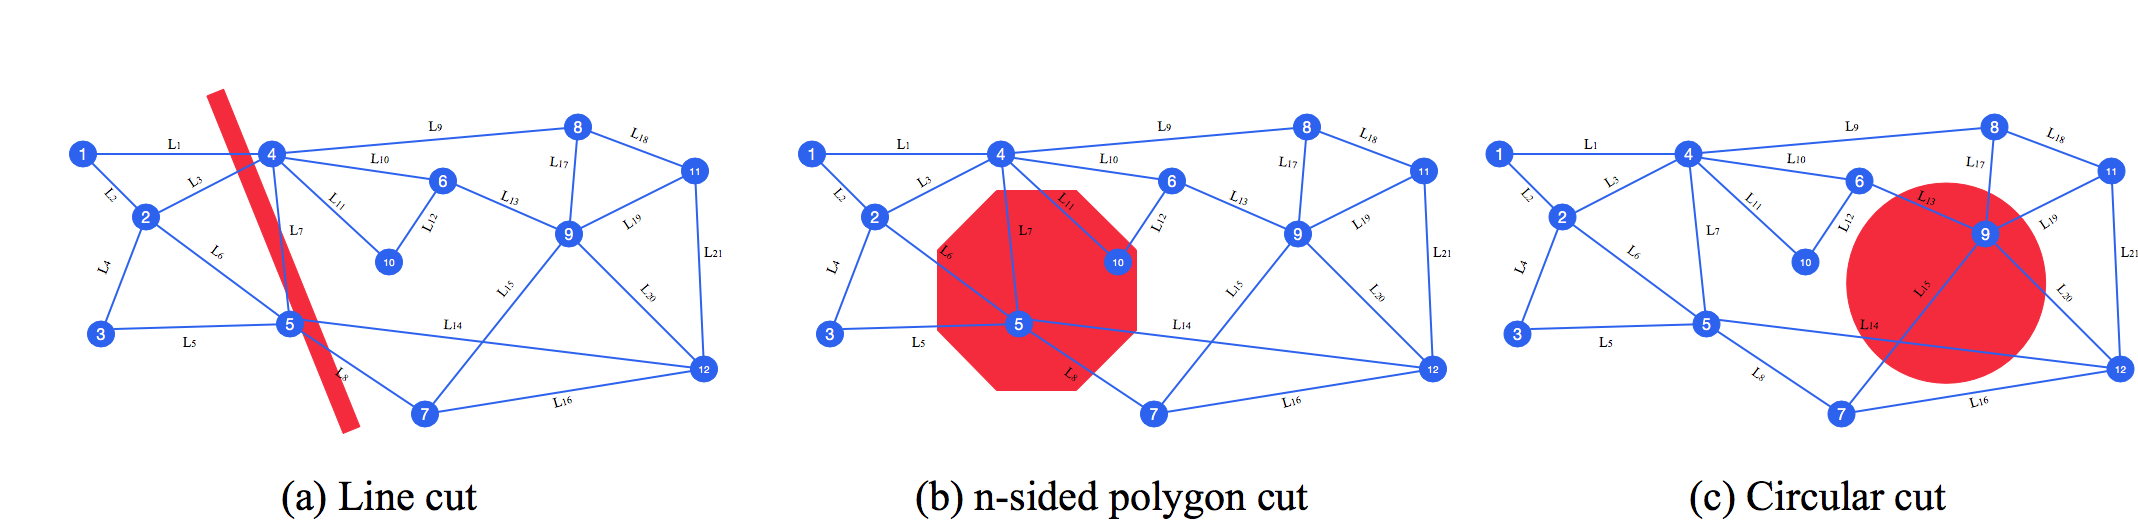
\includegraphics [width=6.5in]{ReginalDemo}
\caption{Disaster region models}
\label{Disaster region models}
\end{figure*}

\par In particular, we can see that the above two equations are equal when p1 = p2 = ... = pn = 1.


\subsection{Mathematical Definition}
\par The main task of this section is to mathematically define regional faults and then to draw a specific description of the problem. In order to describe the problem vividly, we introduce a simple network as an example for illustration.  The simulation experiment uses the backbone network topology of China's three-tier smart grid communication network.  Fig.\ref{G1} shows this topology G1. The radius of the fault marked with a gray shaded area is 100km. The center of fault in this area is (600km, 400km). From the foregoing, we can see that there are many kinds of probability functions of regional failures. We use deterministic  probability functions to visualize the problem. However, when we specifically solve the problem, we comprehensively consider multiple failure probability functions. Table \ref{Definition} shows the definition of mathematical functions and parameters. 
\begin{figure*}[htbp]
\centering
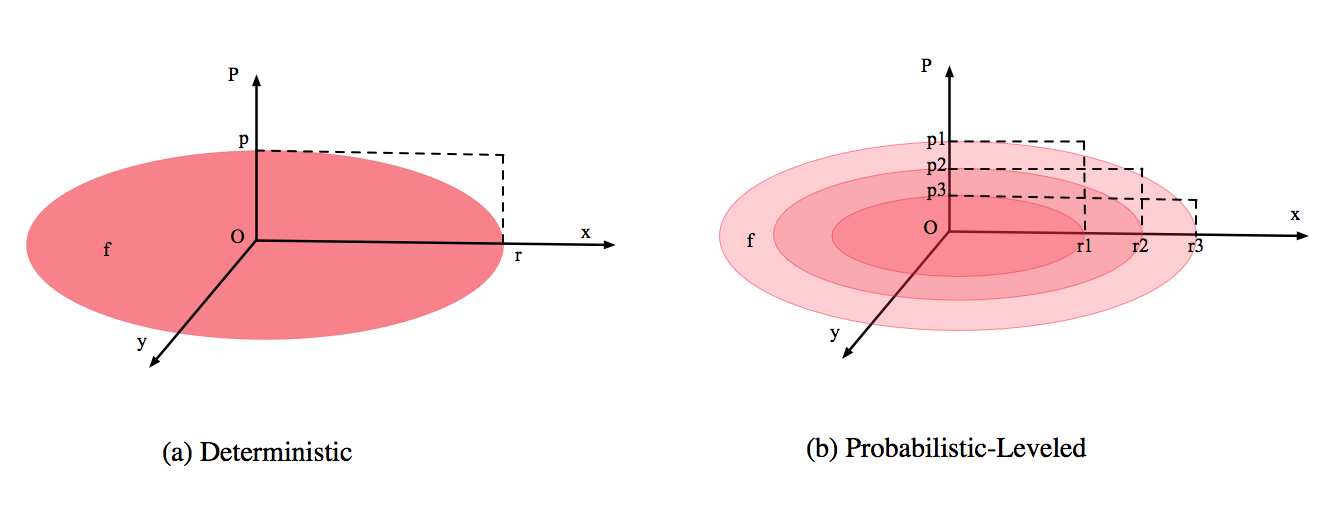
\includegraphics [width=6.5in]{fP}
\caption{Disaster failure probability}
\label{Disaster failure probability}
\end{figure*}
\begin{figure}[htbp]
\centering
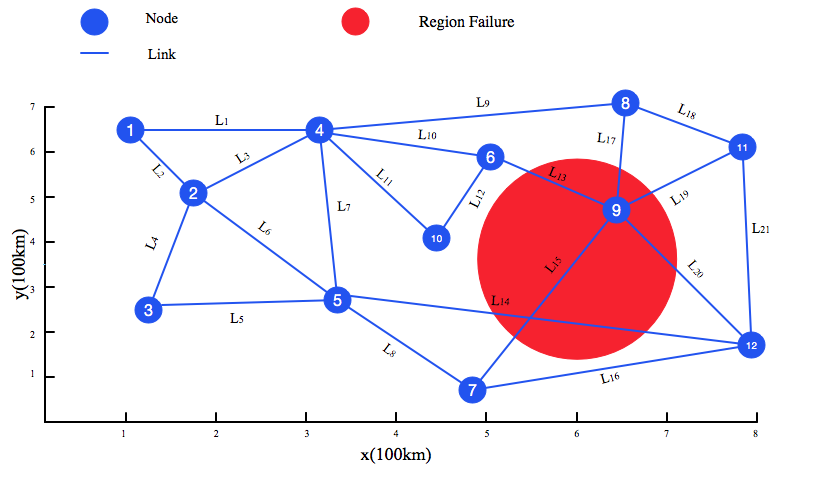
\includegraphics [width=3.5in]{G1}
\caption{G1}
\label{G1}
\end{figure}



\begin{table}[htbp]
\centering
\caption{Definition}
\label{Definition}
\begin{tabular}{@{}
>{\columncolor[HTML]{FFFFFF}}c 
>{\columncolor[HTML]{FFFFFF}}c @{}}
\toprule
Definition & Description                                                                                                                                           \\ \midrule
G(V, E)    & \begin{tabular}[c]{@{}c@{}}G represents the network topology\\ (V represents the nodes set)\\ (E represents the edge set)\end{tabular}                \\ \midrule
q          & the network component (links or nodes)  \\ \midrule
W          & the total cost                                                                                                                                        \\ \midrule
w          & the unit backup cost                                                                                                                                  \\ \midrule
D(G)       & the maximum distance between any two nodes in G                                                                                                       \\ \midrule
f(C, r)   & \begin{tabular}[c]{@{}c@{}}the influence range of the regional fault\\ (C represents the fault center)\\ (r represents the fault radius)\end{tabular} \\ \midrule
P(q, f)          & The probability of failure of q under f \\ \midrule
P(L $|$ f)   & the link(L) is affected by the fault (f) or not                                                                                                       \\ \midrule
PS(L)     & the total number of failures that the link has passed                                                                                                 \\ \midrule
d(f)       & the total number of links in the fault area                                                                                                           \\ \midrule
PSD(L)     & PS(L) combined with fault density                                                                                                \\ \midrule
PSD(E)       & the sum of the PSD(L) of the links in E                                                                                                          \\ \midrule
N(G,f)       & the evaluation of network performance based on f                                                                                                     \\ \midrule
Ew       & the  total number of the workable links in E                                                                                                          \\ \bottomrule


\end{tabular}
\end{table}

\subsubsection{Network Diameter} D(G) refers to the maximum distance between any two nodes in G.

\subsubsection{Binary regional fault function}f (C, r) Indicates the influence range of a regional fault. C indicates the fault center, r indicates the fault radius. The regional fault f1 in Fig.\ref{G1}  can be expressed as follows.
\begin{equation}
f = (C,r)
\end{equation}
\begin{equation}
f1=\left ( C_{1}, 1 \right ),C_{1} = \left ( 6, 4 \right )
\end{equation}
\subsubsection{Link identification function} P(L $|$ f) indicates whether link L is affected by fault f.



\par We can draw the corresponding results of L13, L14, L15, L16 and f1 from Fig.\ref{G1} (L13, L14, L15 are within the f1 range, L16 is not within the f1 range).
\begin{equation}
P(L13|f1) = P(L14|f1) = P(L15|f1) = 1
\end{equation}
\begin{equation}
P(L16|f1) = 0
\end{equation}
\subsubsection{Link failure statistics function} PS (L) indicates how many failures this link may be affected by.
\begin{equation}
PS (L) = \sum_{i=1}^{n} P(L|f_{i})
\end{equation}

\subsubsection{Fault density function} d(f) indicates how many links the fault has passed. This shows the impact of this failure on the entire network. In general, if there is a node in this fault, the area is more dense.
Equation 8 describes d(f1) in G1.
\begin{equation}
d(f) = \sum_{k=1}^{n}P (L_{k} | f)/(f.r)^2
\end{equation}
\begin{equation}
d(f1) = 6/1^{2} = 6
\label{d(f1)}
\end{equation}

\subsubsection{Network evaluation function} N(G, f) indicates the evaluation of network performance based on regional failures. Equation 9 describes N(G, f).

\begin{equation}
N(G,f)=(E_{w}/E)\mid f
\end{equation}
\begin{equation}
E_{w}=workable \quad links \quad in \quad E
\end{equation}
\subsection{Regional Fault}
\par In order to simulate the model, we need to make some constraints on the specific problems and mathematical definitions to get the solution. 
\par First, we use f (C, r) to describe the regional fault. The difficulty of the study is that f is completely random(C and r are randomly chosen in the positive real number domain). In order to reduce the difficulty of solving this problem, we make some weakening constraints on f according to some empirical conditions. For network topology G (V, E), the regional fault f (C, r):
\begin{itemize}
\item For the fault f (C, r), if the distance from C to any node is greater than r, then the fault has no effect on the network. 
\par So we want to get rid of this situation. The mathematical constraint we draw is MIN (C, V) $>$ r.
\item For the fault f (C, r), if r is large, this fault is very destructive and cannot be solved by backup. 
\par Suppose that r $>$=  D(G1)/2 in G1. When c happens randomly, at least one f (C, r) will cover the entire G1. Fig.\ref{AllD} shows that G1 is affected by f(C, r) when r = D (G1)/2. In this case, it is pointless to analyze the network structure because all the links are destroyed by this fault. \par The mathematical constraint we draw is r $<$ 1/2D(G). In general, we simply represent r = D(G)/k, k$>$2.
\begin{figure}[htbp]
\centering
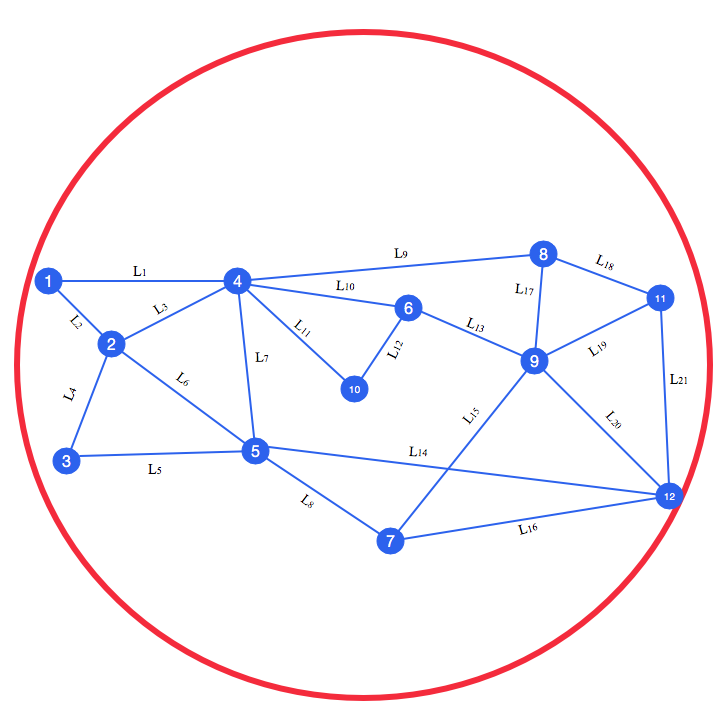
\includegraphics [width=2in]{AllD}
\caption{r = D(G1)/2}
\label{AllD}
\end{figure}
\item Cost constraints. The wireless link has limited communication range. When we back up, we either choose to back up the entire link or choose not to back up. Partial backup of a link is meaningless. In order to simplify the problem, we default the cost of wireless backup only with the link length and wireless transmission.
\end{itemize}

\par From the above constraints, we can draw some important conclusions:

\begin{itemize}
\item In the simulation experiment, we take the fault radius as the input of the algorithm. In the actual environment, the scope of the failure is an important indicator to evaluate the damage of the fault. So we choose fault radius as the core parameter. Different feedback from the network represents resistance to different levels of regional failure.

\item The higher the domain density of the fault area through the link, the lower the resistance. Assume that only two fault zones f1 and f2 are considered, as shown in Fig.\ref{f1f2}. 
\begin{figure}[htbp]
\centering
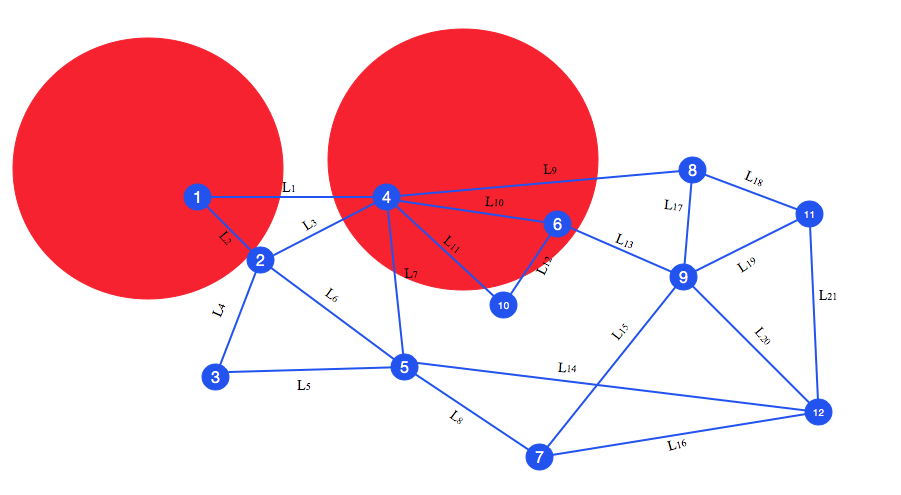
\includegraphics [width=3in]{f1f2}
\caption{two fault zones}
\label{f1f2}
\end{figure}
\begin{equation}
PS (L2) = P(L2|f1) + P(L2|f2) = 1
\end{equation}
\begin{equation}
PS (L12) = P(L12|f1) + P(L12|f2) = 1
\end{equation}
\par Because of PS (L2) = PS (L12), we should randomly select a link for backup. But d(f1) = 2 $<$ d(f2) = 7, this shows that f2 causes more link failures. So L12 should take precedence over L2. In other words, L12 is more likely to be in the center of the network. 
\end{itemize}
\par So we introduce the PSD(L) and PSD(E) (E represents the link set). The smaller the PSD function value, the greater its network resistance.
\begin{equation}
PSD (L) = \sum_{i=1}^{n} P(L|f_{i})\cdot  d(f_{i})
\end{equation}
\begin{equation}
PSD (E) = \sum_{E} PSD(L)
\end{equation}

\subsection{Problem model}
\par For network G and P(q, f), we need to find the result set R to satisfy the following three formulas (E represents the link set of G, W represents the total cost, w represents the unit cost).
\begin{equation}
R\subseteq E
\end{equation}
\begin{equation}
wR <= W
\end{equation}
\begin{equation}
min (PSD (E-R))
\end{equation}
\par The above constraint indicates that we require a set of edges that satisfy the cost constraint. This set will minimize the set of PSD functions for the remaining edges. We explain the algorithm in the next chapter.

\section{Algorithm}
\par In order to solve the problem in the previous section, we propose a region-based fault tolerant algorithm based on sampling points (SPA).
\par Before describing the SPA, we must first determine the simulation method of regional failure. The more sampling points we choose, the more accurate data we draw. However, due to the constraints of the actual environment and simulation conditions, this article selects the sampling points according to the specific conditions of the topology.
\subsection{Simulation method}
\begin{figure}[htbp]
\centering
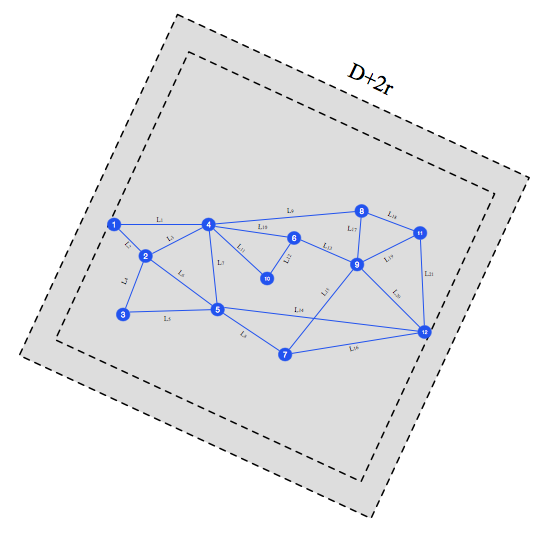
\includegraphics [width=2.8in]{d+2r}
\caption{sampling ranges}
\label{d+2r}
\end{figure}
\subsubsection{Sampling range}It is the range affected by the fault. In Fig. \ref{d+2r}, D is the diameter of the network and r is the radius of the fault. The area of the dotted line enclosed by a square of length D + 2r in the figure can be regarded as the domain of the fault center point. We can prove that the failure of the area may affect the topology only when the fault center is in the domain [15]. Otherwise, the shortest distance from the node to the topology is longer than the fault radius. 
\subsection{Specific algorithm}
\par First, we show the meaning of the input parameters of the algorithm. G represents the network topology, V represents the network node set, E represents the network edge set, W represents the total cost, w represents the unit backup cost, r represents the fault radius. The result given by the algorithm is denoted R. See the appendix for the specific algorithm. SPA is divided into two phases. For the convenience of explanation, we combine the algorithm steps to explain concretely.
 
\subsubsection{Sample point generation phase}
\par This section takes G0 as an example to illustrate the concrete realization of the algorithm. Fig.\ref{G0} shows the topology of G0. We assume that the fault radius is 1km. Fig.\ref{Calculate network diameter} shows the calculation of network diameter. Fig.\ref{Generate sampling points} shows the sampling point generation process. 

\begin{figure}[htbp]
\centering
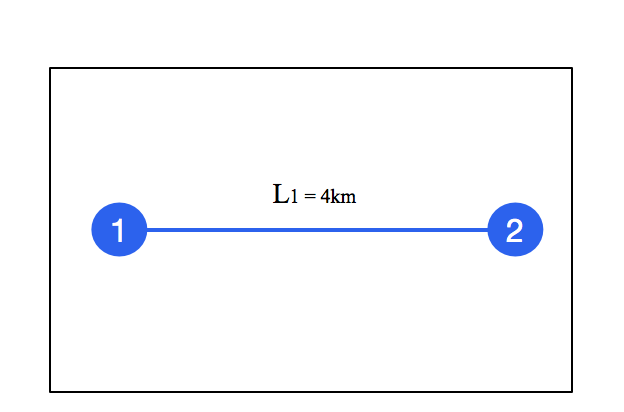
\includegraphics [width=2in]{G0}
\caption{G0}
\label{G0}
\end{figure}
\begin{figure}[htbp]
\centering
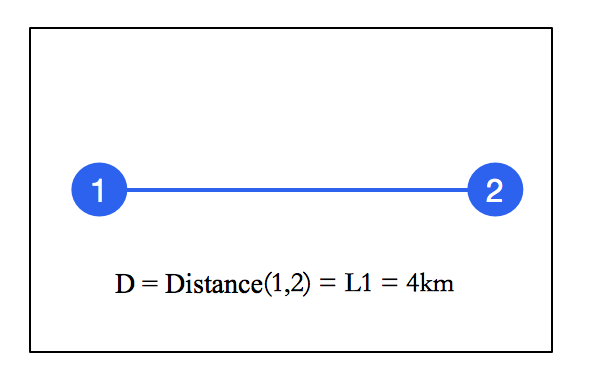
\includegraphics [width=2in]{G0S1C}
\caption{Calculate network diameter}
\label{Calculate network diameter}
\end{figure}
\begin{figure}[htbp]
\centering
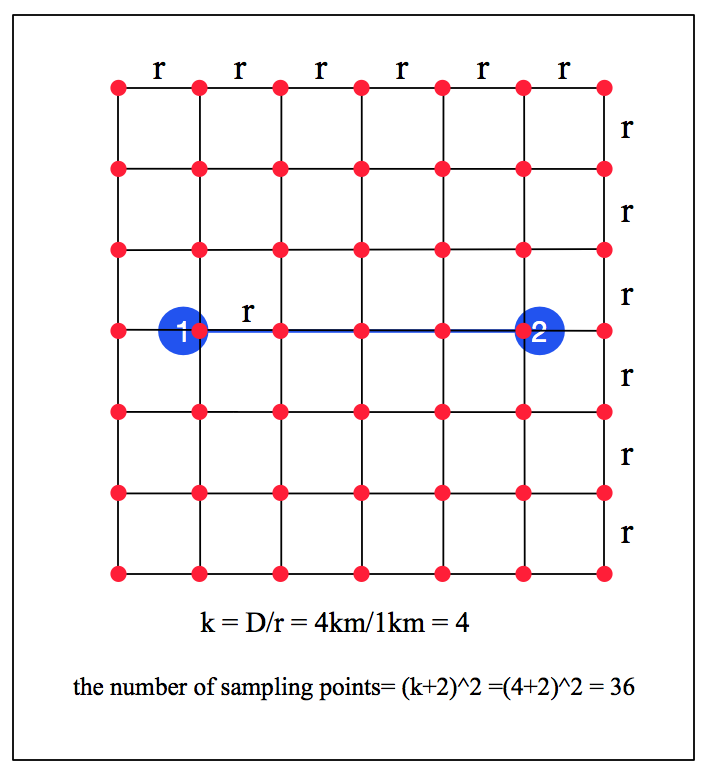
\includegraphics [width=2.8in]{G0S1G}
\caption{Generate sampling points}
\label{Generate sampling points}
\end{figure}


\subsubsection{Link inspection phase}
\par Fig.\ref{Link inspection} shows how to calculate the relationship between link and fault and how to generate the result. 


\begin{figure}[htbp]
\centering
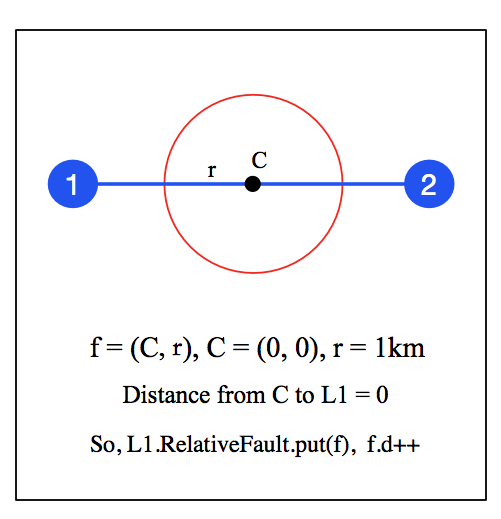
\includegraphics [width=2.4in]{G0S2F}
\caption{Link inspection}
\label{Link inspection}
\end{figure}


 \section{Simulation experiment}
 \par This paper uses the NetworkX simulation package to generate an emulation network and performs simulation experiments on this platform [16]. NetworkX is a Python package for the creation, manipulation, and study of the structure, dynamics, and functions of complex networks. The purpose of the experiment is to validate the model and verify the algorithm. As shown in Fig.\ref{Simulation Network G1}, we use G1 as the simulation network. 
 
 
\begin{figure}[htbp]
\centering
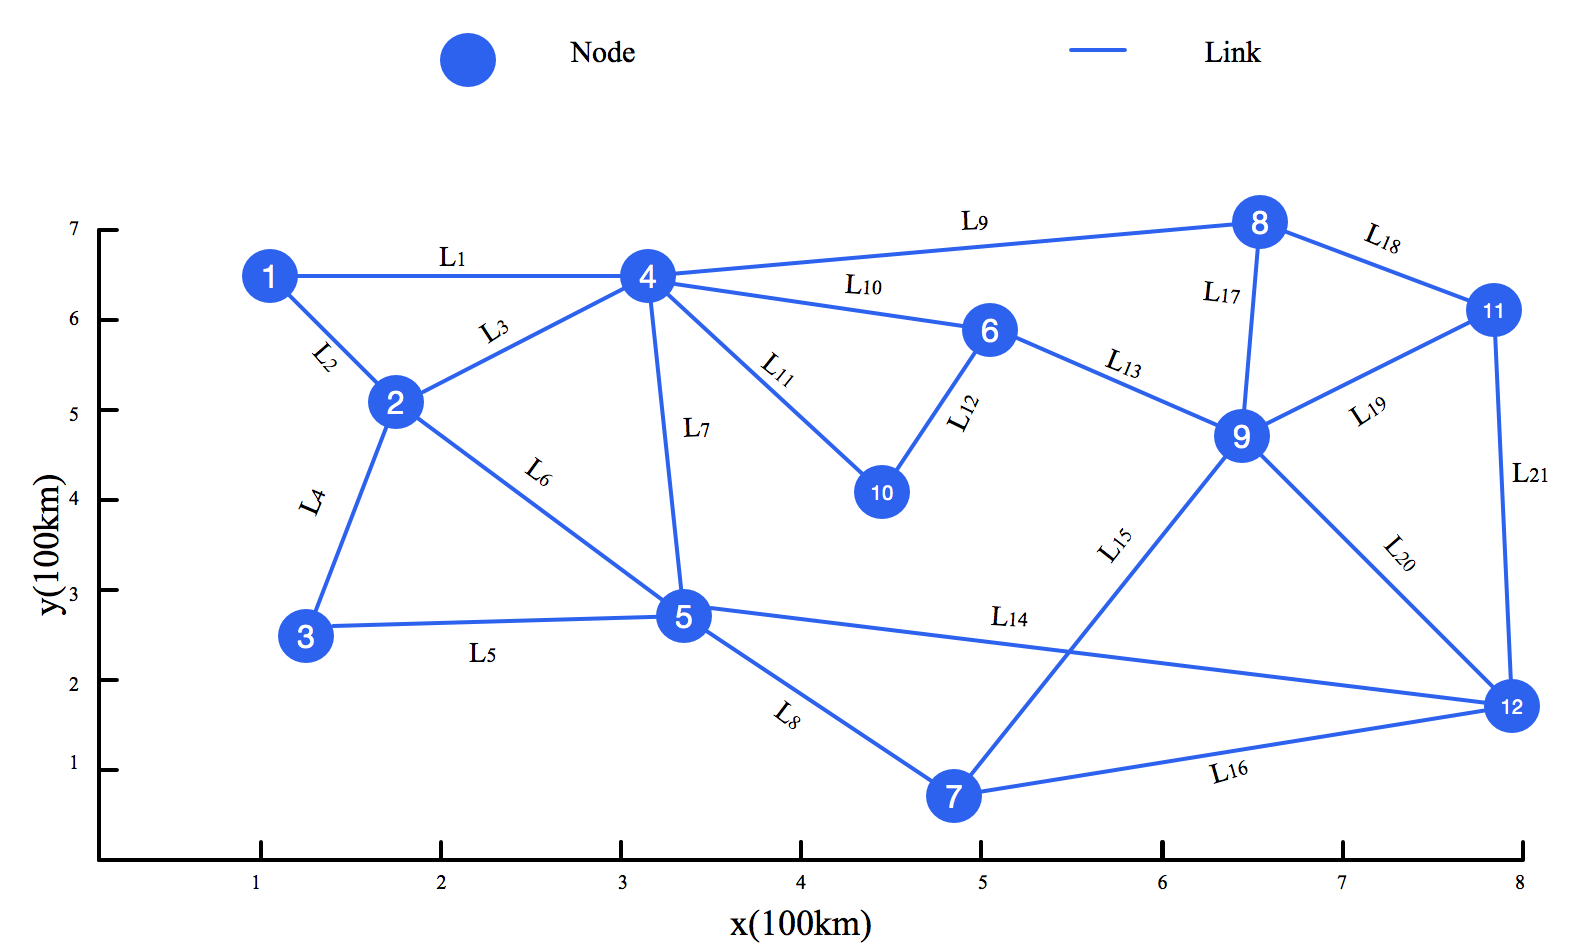
\includegraphics [width=2.8in]{G1S}
\caption{Simulation Network G1}
\label{Simulation Network G1}
\end{figure}
 \subsection{Comparison algorithm}
\par Next, we introduce the comparison algorithm. At present, some algorithms have been proposed for the study of regional faults, and this part has already been partly explained in the previous section. We chose two algorithms in this section as the control group for the experimental effect. LSRA (Landmark-based Source Routing Algorithm) [17] uses the geographically distributed intermediate nodes, named landmarks, to reestablish the connection through a shortest path. PRFAA (Probabilistic Region Failure-Aware Algorithm) proposes an Integer Linear Program-based theoretical framework to identify the optimal data center network placement to lead to the minimum data center network failure risk under a region failure [18]. 
  \subsection{SPA}
According to the algorithm, we can draw the following data. As shown in Fig.\ref{Diameter}, we can get the diameter of the network through the algorithm. After that we explained the specific calculation process.
\begin{figure}[htbp]
\centering
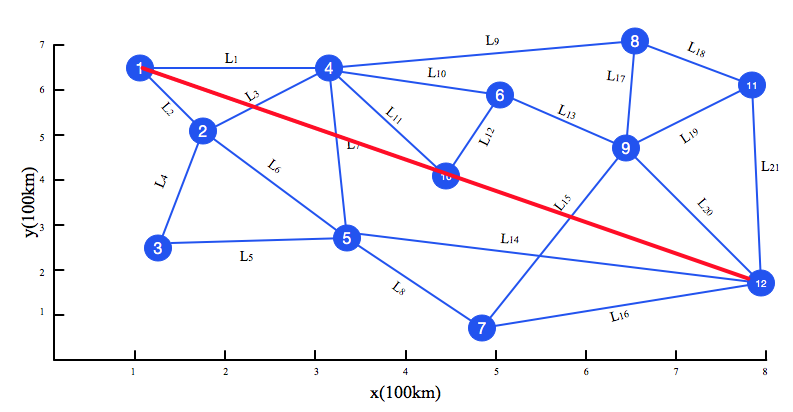
\includegraphics [width=3in]{Distance}
\caption{Diameter}
\label{Diameter}
\end{figure}
\begin{equation}
D=Distance\left ( node1, node12  \right ) 
\end{equation}
\begin{equation}
D= \sqrt{(node1.x- node12.x)^{2} + (node1.y- node12.y)^{2}}
\end{equation}
\begin{equation}
D= \sqrt{(1- 8)^{2} + (6.5- 2)^{2}} = 8.32
\end{equation}

\par As shown in Fig.\ref{d6}, We show the sampling points when r = D/6 =1.39.
\begin{figure}[htbp]
\centering
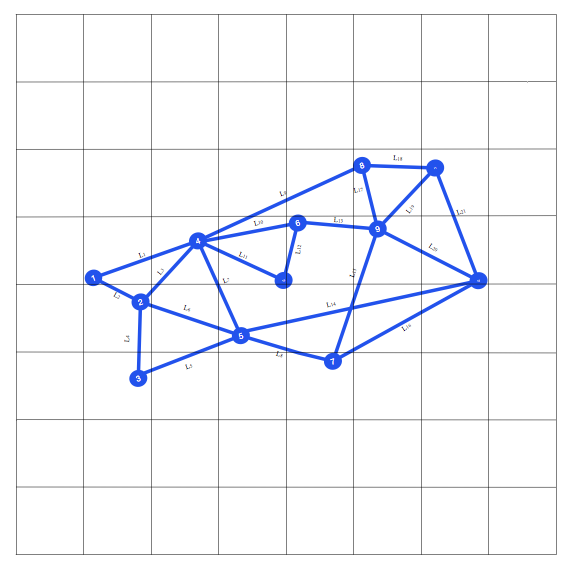
\includegraphics [width=2in]{d6}
\caption{r = D/6}
\label{d6}
\end{figure}
 \subsection{Algorithm evaluation}
 \par Due to the particularity of regional faults, we take the total cost and the radius of regional faults as input parameters. Fig.\ref{Fault} shows the difference in performance between algorithms when input parameters change. R0, R1 and R2 in the Fig.\ref{Fault} show different fault radiuses (R1 = D/6 = 1.39 and R2 = D/4 = 2.08). The abscissa of the Fig.\ref{Fault} indicates the proportion of the backup link(10\%-75\%). This parameter is proportional to W/w. In simulation experiments, we considered the following two kinds of probability functions respectively.
 

\begin{equation}
P_{1}\left ( q, f \right )=\left\{\begin{matrix}
1,\, \, if \, q \, instersects \, f\,within \, r/2 \,\,\,\,\,\,\,\,\,\,\,\,\,\,\,\,\,\,\,\, \, \,\,\,\,\,\,\,\, \,\\ 
0.5,\, \, if \, q \, instersects \, f\,between \,r/2 \, and \, r \,\,\,\,\,\,\,\,\, \, \,& \\ 
0,\, \, \, \,\, \,otherwise \,\,\,\,\,\,\,\,\,\,\, \,\,\,\,\,\,\,\,\,\,\,\,\,\,\,\,\,\,\,\,\,\,\,\,\,\,\,\,\,\,\,\,\,\,\,\,\,\,\,\,\,\,\,\,\,\,\,\,\,\,\,\,\,\,\,\,\,\,&  
\end{matrix}\right.
\end{equation}
  \begin{equation}
P_{2}\left ( q, f \right )=\left\{\begin{matrix}
1, if \, q \, instersects \, f\, & \\ 
0,  \,\,\,\,\,\,\,\,\,\,\,\,\,\,\,\,\,\,\,  otherwise & 
\end{matrix}\right.
\end{equation}
\par We can draw the following conclusions based on the simulation results.
\begin{itemize}
\item The backup algorithm proposed in this paper effectively improves the robustness of the network against regional failures.
\item As the radius of regional failure increases, the damage to the network is greater.
\item The probability function of different regional failures has different degrees of influence on the robustness of the network. The proposed algorithm shows better performance under various probability functions.

\end{itemize}
 \begin{figure*}[htbp]
\centering   
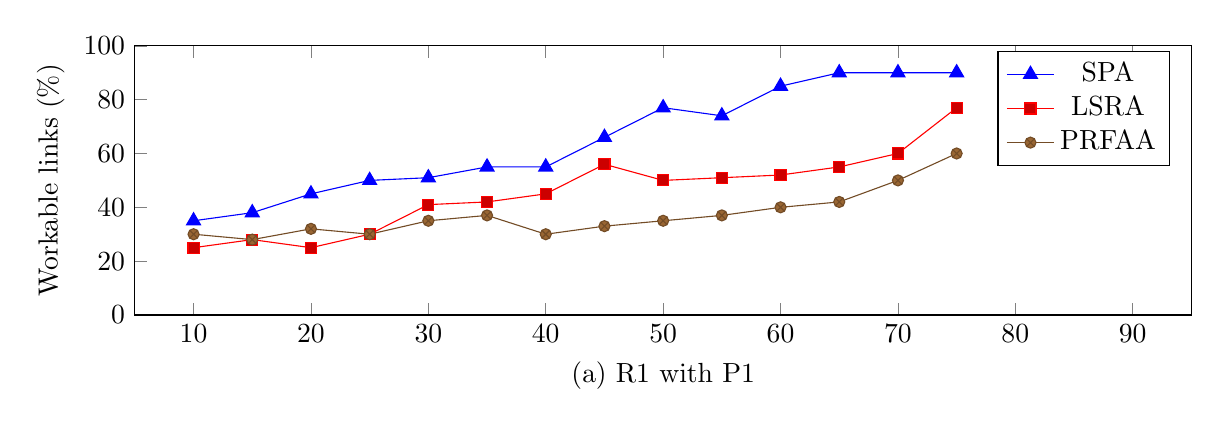
\begin{tikzpicture}
\begin{axis}
[
height=5cm,
width=15cm,
xlabel=(a) R1 with P1,
ylabel=Workable links (\%),
xmin=5,
xmax=95,
ymin=0,
ymax=100,
ytick pos=left
]
\addplot[color=blue,
    mark=triangle*, mark size=2.9pt ] coordinates {
(10,   35)(15,   38)
(20,   45)(25,   50)
(30,   51)(35,   55)
(40,   55)(45,   66)
(50,   77)(55,   74)
(60,   85)(65,   90)
(70,   90)(75,   90)

};
\addlegendentry{SPA}

\addplot coordinates {
(10,   25)(15,   28)
(20,   25)(25,   30)
(30,   41)(35,   42)
(40,   45)(45,   56)
(50,   50)(55,   51)
(60,   52)(65,   55)
(70,   60)(75,   77)

};

\addlegendentry{LSRA}

\addplot coordinates {
(10,   30)(15,   28)
(20,   32)(25,   30)
(30,   35)(35,   37)
(40,   30)(45,   33)
(50,   35)(55,   37)
(60,   40)(65,   42)
(70,   50)(75,   60)

};
\addlegendentry{PRFAA}
\end{axis}
\end{tikzpicture}
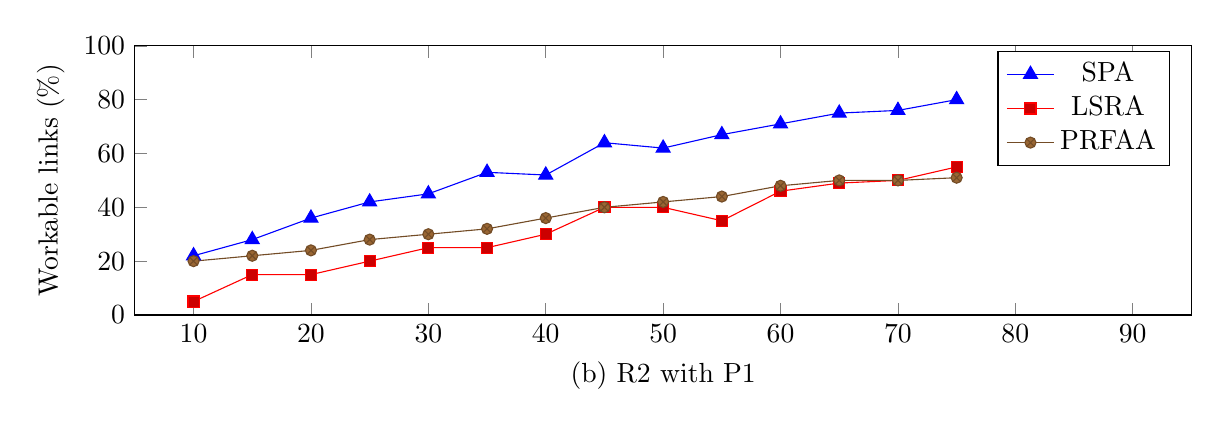
\begin{tikzpicture}
\begin{axis}
[
height=5cm,
width=15cm,
xlabel=(b) R2 with P1,
ylabel=Workable links (\%),
xmin=5,
xmax=95,
ymin=0,
ymax=100,
ytick pos=left
]
\addplot[color=blue,
    mark=triangle*, mark size=2.9pt ] coordinates {
(10,   22)(15,   28)
(20,   36)(25,   42)
(30,   45)(35,   53)
(40,   52)(45,   64)
(50,   62)(55,   67)
(60,   71)(65,   75)
(70,   76)(75,   80)

};
\addlegendentry{SPA}

\addplot coordinates {
(10,   5)(15,   15)
(20,   15)(25,   20)
(30,   25)(35,   25)
(40,   30)(45,   40)
(50,   40)(55,   35)
(60,   46)(65,   49)
(70,   50)(75,   55)

};

\addlegendentry{LSRA}

\addplot coordinates {
(10,   20)(15,   22)
(20,   24)(25,   28)
(30,   30)(35,   32)
(40,   36)(45,   40)
(50,   42)(55,   44)
(60,   48)(65,   50)
(70,   50)(75,   51)

};
\addlegendentry{PRFAA}
\end{axis}
\end{tikzpicture}

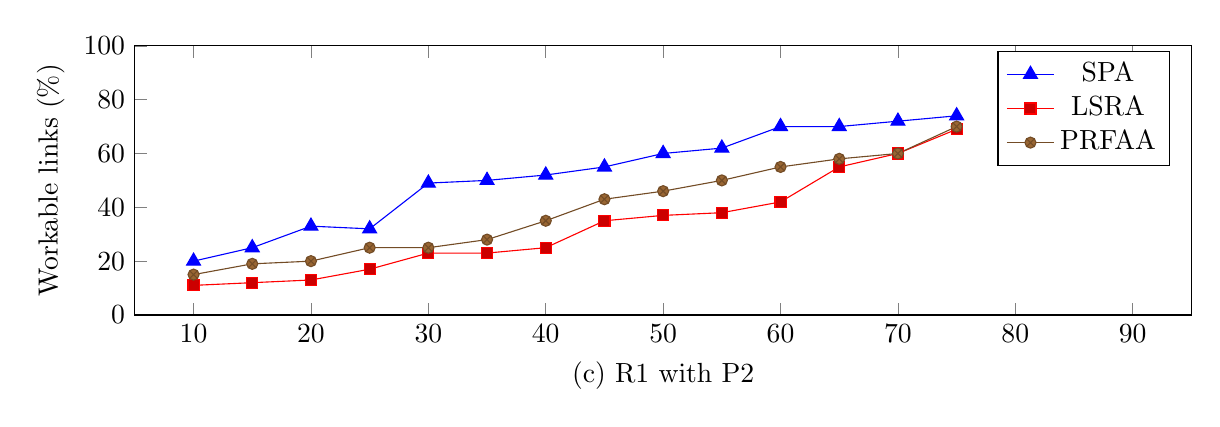
\begin{tikzpicture}
\begin{axis}
[
height=5cm,
width=15cm,
xlabel=(c) R1 with P2,
ylabel=Workable links (\%),
xmin=5,
xmax=95,
ymin=0,
ymax=100,
ytick pos=left
]
\addplot[color=blue,
    mark=triangle*, mark size=2.9pt ] coordinates {
(10,   20)(15,   25)
(20,   33)(25,   32)
(30,   49)(35,   50)
(40,   52)(45,   55)
(50,   60)(55,   62)
(60,   70)(65,   70)
(70,   72)(75,   74)

};
\addlegendentry{SPA}

\addplot coordinates {
(10,   11)(15,   12)
(20,   13)(25,   17)
(30,   23)(35,   23)
(40,   25)(45,   35)
(50,   37)(55,   38)
(60,   42)(65,   55)
(70,   60)(75,   69)

};

\addlegendentry{LSRA}

\addplot coordinates {
(10,   15)(15,   19)
(20,   20)(25,   25)
(30,   25)(35,   28)
(40,   35)(45,   43)
(50,   46)(55,   50)
(60,   55)(65,   58)
(70,   60)(75,   70)

};
\addlegendentry{PRFAA}\end{axis}
\end{tikzpicture}
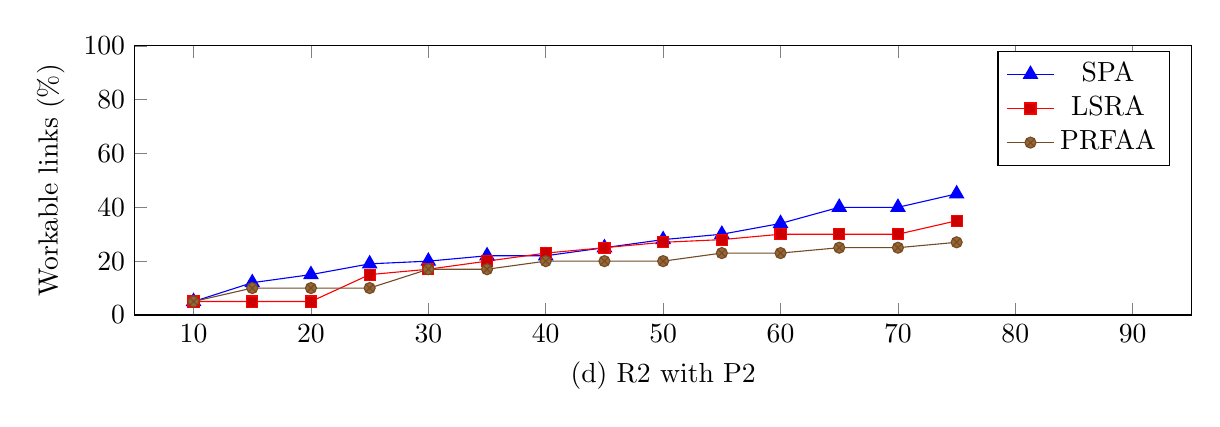
\begin{tikzpicture}
\begin{axis}
[
height=5cm,
width=15cm,
xlabel=(d) R2 with P2,
ylabel=Workable links (\%),
xmin=5,
xmax=95,
ymin=0,
ymax=100,
ytick pos=left
]
\addplot[color=blue,
    mark=triangle*, mark size=2.9pt ] coordinates {
(10,   5)(15,   12)
(20,   15)(25,   19)
(30,   20)(35,   22)
(40,   22)(45,   25)
(50,   28)(55,   30)
(60,   34)(65,  40)
(70,   40)(75,   45)
};
\addlegendentry{SPA}

\addplot coordinates {
(10,   5)(15,   5)
(20,   5)(25,   15)
(30,   17)(35,   20)
(40,   23)(45,   25)
(50,   27)(55,   28)
(60,   30)(65,   30)
(70,   30)(75,   35)

};

\addlegendentry{LSRA}

\addplot coordinates {
(10,   5)(15,   10)
(20,   10)(25,   10)
(30,   17)(35,   17)
(40,   20)(45,   20)
(50,   20)(55,   23)
(60,   23)(65,   25)
(70,   25)(75,   27)

};
\addlegendentry{PRFAA}\end{axis}
\end{tikzpicture}
\caption{Simulation results} %                         %????
\label{Fault}
\end{figure*}


\section{Conclusion}
\par SPA has shown higher performance than other algorithms in terms of tolerating regional failures. Currently, algorithms used in the field of fault tolerance either have insufficient analysis of regional failures or have not been optimized accordingly for regional failures. The comparison algorithm performs poorly in the transmission of faults in areas with larger radii(multiple mark paths will be destroyed). The node sampled by the SPA calculates the importance of each node. We use this to make more accurate node backups.
\par In particular, SPA is based on the analysis and simulation of the topology in this paper. If you want to confirm the performance of this algorithm, you can analyze it by adjusting the network topology results and the regional failure probability function.


\section*{Acknowledgment}

The work is supported by National Natural Science Foundation of China (61302078, 61372108), 863 Program (2011AA01A102), Funds for Creative Research Groups of China (61121061).
% if have a single appendix:
%\appendix[Proof of the Zonklar Equations]
% or
%\appendix  % for no appendix heading
% do not use \section anymore after \appendix, only \section*
% is possibly needed

% use appendices with more than one appendix
% then use \section to start each appendix
% you must declare a \section before using any
% \subsection or using \label (\appendices by itself
% starts a section numbered zero.)
%


% Can use something like this to put references on a page
% by themselves when using endfloat and the captionsoff option.
\newpage
\begin{thebibliography}{1}

\bibitem{IEEEhowto:kopka}
M. F. Habib, M. Tornatore, F. Dikbiyik, and B. Mukherjee, Disaster survivability in optical communication networks, Comput. Commun.,vol. 36, no. 6, pp. 630–644, Mar. 2013.
\bibitem{IEEEhowto:kopka}
X. Huang, Y. J. Guo, A. Zhang, and V. Dyadyuk, A multi-gigabit microwave backhaul, IEEE Commun. Mag., vol. 50, no. 3, pp. 122–129, Mar. 2012.
\bibitem{IEEEhowto:kopka}
P. K. Agarwal, A. Efrat, S. K. Ganjugunte, D. Hay, S. Sankararaman, and G. Zussman, The resilience of WDM networks to probabilistic geographical failures, IEEE/ACM Trans. Netw., vol. 21, no. 5, pp. 1525–1538, Oct. 2013.
\bibitem{IEEEhowto:kopka}
Q. Zheng, G. Cao, T. L. Porta, and A. Swami, Optimal recovery from large-scale failures in ip networks, in IEEE International Conference on Distributed Computing Systems (ICDCS), 2012.
\bibitem{IEEEhowto:kopka}
Zhao, L., et al. (2013). Power and bandwidth efficiency of
wireless mesh networks. IET Networks, 2(3), 131–140.
\bibitem{IEEEhowto:kopka}
Vural, S., et al. (2013). Survey of experimental evaluation studies for wireless mesh network deployments in urban areas towards ubiquitous Internet. IEEE Communications Surveys and Tutorials, 15(1), 223–239.
\bibitem{IEEEhowto:kopka}

Li, H., et al. (2013). Routing metrics for minimizing end-to-end delay in multiradio multichannel wireless networks. IEEE Transactions on Parallel and Distributed Systems, 24(11), 2293–2303.
\bibitem{IEEEhowto:kopka}
Paris, S., et al. (2013). Cross-layer metrics for reliable routing in wireless mesh networks. IEEE/ACM Transactions on Networking, 21(3), 1003–1016.
\bibitem{IEEEhowto:kopka}
A. Leonardi, K. Mathioudakis, A. Wiesmaier, and F. Zeiger. (2014, Aug.). Towards the smart grid: Substation automation architecture and technologies. Advances in Electrical Engineering. [Online]. 2014(2014),
pp. 1–13.
\bibitem{IEEEhowto:kopka}
Y. Q. Liu, H. L. Gao, W. C. Gao, and F. Peng, Development of a substation-area backup protective relay for smart substation, IEEE Transactions on Smart Grid, vol. PP, no. 99, pp. 1–10, Feb. 2016.
\bibitem{IEEEhowto:kopka}
Xiaoliang Wang; Xiaohong Jiang; Cam-Tu Nguyen; Xiao Zhang; Sanglu Lu, Fast connection recovery against region failures with landmark-based source routing, 2013 9th International Conference on the Design of Reliable Communication Networks (DRCN).
\bibitem{IEEEhowto:kopka}
Yazan M. Allawi; Dujeong Lee; June-Koo Kevin Rhee, A Wireless Link-Up Augmentation Design for Disaster-Resilient Optical Networks, Journal of Lightwave Technology, 2015.
\bibitem{IEEEhowto:kopka}
János Tapolcai; Lajos Rónyai; Balázs Vass; László Gyimóthi, List of shared risk link groups representing regional failures with limited size, IEEE INFOCOM 2017 - IEEE Conference on Computer Communications, 2017.
\bibitem{IEEEhowto:kopka}

Carlos Galdamez; Zilong Ye, Resilient virtual network mapping against large-scale regional failures, 2017 26th Wireless and Optical Communication Conference (WOCC).
\bibitem{IEEEhowto:kopka}
Xiao Liu; Ying Wang; Ailing Xiao; Xuesong Qiu; Wenjing Li, Disaster-prediction based virtual network mapping against multiple regional failures, 2015 IFIP/IEEE International Symposium on Integrated Network Management (IM).
\bibitem{IEEEhowto:kopka}


Hongfang Yu; Chunming Qiao; Jianping Wang; Lemin Li; Vishal Anand; Bin Wu, Regional failure-resilient virtual infrastructure mapping in a federated computing and networking system, IEEE/OSA Journal of Optical Communications and Networking, 2014.



\bibitem{IEEEhowto:kopka}

Xu Zhang; Shuai Yue; Xiaobing Zha, Method of power grid fault diagnosis using intuitionistic fuzzy Petri nets, IET Generation, Transmission & Distribution, 2018.
\bibitem{IEEEhowto:kopka}
Stefan Hosein; Patrick Hosein; Walter Kattick; Varma Ratan, Web application for power grid fault management, 2016 6th International Conference on Intelligent and Advanced Systems (ICIAS).
\end{thebibliography}
 
 
 
 
 
 
 
 
 
 
 
\newpage
\begin{appendix}  
\section{1}  
\begin{algorithm}
        \caption{SPA}
        \begin{algorithmic}[1] %??????
            \Require G, V, E, W, w, r, P(q, f)
            \Ensure R
            \State \textbf{global} $ArrayFault\gets 0$
             \State \textbf{global} $R\gets 0$
            \State \textbf{global} $k\gets 0$
             \Function {Main}{$G$}
              
                \State $D\gets $\Call{GenerateDiameter}{$V$}
                \State $\Call {GenerateFaultSet}{$D,V, r$} $

	        \State $\Call{CheckInFault}{$E$} $
		\State $E.orderBy(L.psd)$

                \For {$ L : E $}
		\If {$W > wL $}
			\State $R .put(L)$
			\State $W \gets W - wL$
		\EndIf
\EndFor 
                 \State \Return{$R$}
            \EndFunction
            
            
            
            
            \Function {GenerateDiameter}{$V, r$}
           	 \State $D.length\gets 0$
            	 \For{$head:V$}
	  		\For{$tail:V$}
				 \State $length \gets \Call{Distance}{$head, tail$}$
				\If{$ length > D.length$}
				 	\State $D.length \gets length$
				  	\State $D.head \gets head$
				 	 \State $D.tail \gets tail$
				\EndIf
			\EndFor 
		\EndFor 
		 \State $k\gets D/r$     
		 \State \Return{$D$}      
            \EndFunction
            \Function {GenerateFaultSet}{$D,V, r$}
            	\State $origin \gets (head + tail - D - 2r) / 2 $
		
	 	 \For{$i:  range (k + 2)$}
	  		\For{$j :  range (k + 2)$}
				 \State $fault \gets (C(origin.x + i * r, origin.x + j * r) r)$
				\State $ArrayFault.append(fault)$
			\EndFor 
		\EndFor   
            \EndFunction
                    \end{algorithmic}
    \end{algorithm}
          \begin{algorithm}
        \caption{SPA-CheckInFault}
        \begin{algorithmic}[1] %??????   
             \Function {CheckInFault}{$E$}
            	\State $origin \gets (head + tail - D - 2r) / 2 $
		
	 	 \For{$L :  E$}
	  		\For{$f : ArrayFault$} 
				\State $O \gets f.c $
				\State $H \gets L.head $
				\State $L \gets L.tail $
				
				\State $OH \gets \Call{Distance}{$O, H$}$
				\State $HL \gets \Call{Distance}{$H, L$}$
				\State $OL \gets \Call{Distance}{$O, L$}$
				\State $S \gets \Call{Distance}{$S, HL$}$
				
				

				 \If{ \Call{Check}}
					\State $L.RelativeFault.put(f)$
				  	\State $f.d  ++$				 				
				\EndIf
			\EndFor 
			 \For{$L :  E$}	  	
					\State $L.psd \gets L.RelativeFault.sum$
			\EndFor 
		\EndFor
		\Function {Check}{}
		\If{$ Math.Random() \,not \, in \,P(q, f)$}
		    \State \Return{$False$} 
		\EndIf
		
		\If{$ sign(OH - r) \& sign(OT - r)$}
		\State $Angle \gets sign(OH^2+HT^2-OT^2) (OT^2+HT^2-OH^2) $
		 \State \Return{Angle\&(sign(r-S))}
		\Else
			\State \Return{$True$}      
		\EndIf
		\EndFunction
            \EndFunction
             
           
            
        \end{algorithmic}
    \end{algorithm}

\end{appendix}  
% trigger a \newpage just before the given reference
% number - used to balance the columns on the last page
% adjust value as needed - may need to be readjusted if
% the document is modified later
%\IEEEtriggeratref{8}
% The "triggered" command can be changed if desired:
%\IEEEtriggercmd{\enlargethispage{-5in}}

% references section

% can use a bibliography generated by BibTeX as a .bbl file
% BibTeX documentation can be easily obtained at:
% http://mirror.ctan.org/biblio/bibtex/contrib/doc/
% The IEEEtran BibTeX style support page is at:
% http://www.michaelshell.org/tex/ieeetran/bibtex/
%\bibliographystyle{IEEEtran}
% argument is your BibTeX string definitions and bibliography database(s)
%\bibliography{IEEEabrv,../bib/paper}
%
% <OR> manually copy in the resultant .bbl file
% set second argument of \begin to the number of references
% (used to reserve space for the reference number labels box)


% biography section
% 
% If you have an EPS/PDF photo (graphicx package needed) extra braces are
% needed around the contents of the optional argument to biography to prevent
% the LaTeX parser from getting confused when it sees the complicated
% \includegraphics command within an optional argument. (You could create
% your own custom macro containing the \includegraphics command to make things
% simpler here.)
%\begin{IEEEbiography}[{\includegraphics[width=1in,height=1.25in,clip,keepaspectratio]{mshell}}]{Michael Shell}
% or if you just want to reserve a space for a photo:



% You can push biographies down or up by placing
% a \vfill before or after them. The appropriate
% use of \vfill depends on what kind of text is
% on the last page and whether or not the columns
% are being equalized.

%\vfill

% Can be used to pull up biographies so that the bottom of the last one
% is flush with the other column.
%\enlargethispage{-5in}



% that's all folks
\end{document}


